\documentclass[english,12pt]{article}
\usepackage[T1]{fontenc}
\usepackage{geometry}
\geometry{verbose,bmargin=2.5cm,lmargin=2.5cm,rmargin=2.5cm}
\usepackage[utf8]{inputenc}
\usepackage{amsmath}
\usepackage{amsfonts}
\usepackage{amssymb}
\usepackage{rotfloat}
\usepackage{wasysym}
\usepackage{graphicx}
\usepackage{natbib}
\usepackage{latexsym}
\usepackage{caption}
\usepackage{flafter}
\usepackage{babel}
\usepackage{imakeidx}
\usepackage{amssymb,amsmath}
\usepackage[table]{xcolor}
\usepackage[mathlines,displaymath]{}
\usepackage{anyfontsize}
\usepackage{verbatim}

\newcommand{\etal}{{et~al.{}}}
\newcommand{\ie}{{i.~e.{}}}
\newcommand{\eg}{{e.~g.{}}}
\newcommand{\viz}{{viz.{}}}
\newcommand{\etc}{{etc.{}}}
\newcommand{\apriori}{{a priori{}}}
\newcommand{\vv}{{vice versa{}}}
\newcommand{\cf}{{}}
\usepackage{titling}
\usepackage{color}


\date{}

\topmargin 0.0cm
\oddsidemargin 0.5cm
\evensidemargin 0.5cm
\textwidth 16cm 
\textheight 22cm

\makeindex
\begin{document}

\begin{flushleft}
\textbf{\Large {$\mathcal{ROBHOOT}$} -- An Open Platform To Investigate Investment Markets}
%by $\mathcal{N}$+3 -- {\small Computing worldwide access to ideas}}
\\
\vspace{1.0cm} Alejandro Rozenfeld$^{1}$, Charles N. de Santana$^{1}$, Carlos J. Meli\'an$^{1}$
\\
\vspace{1.0cm} \bf{1} Horizontal Networks Center. Infinite Galaxy Road, Via Lactea.
\\
\begin{figure}
\vspace{-3 in}
\begin{center}
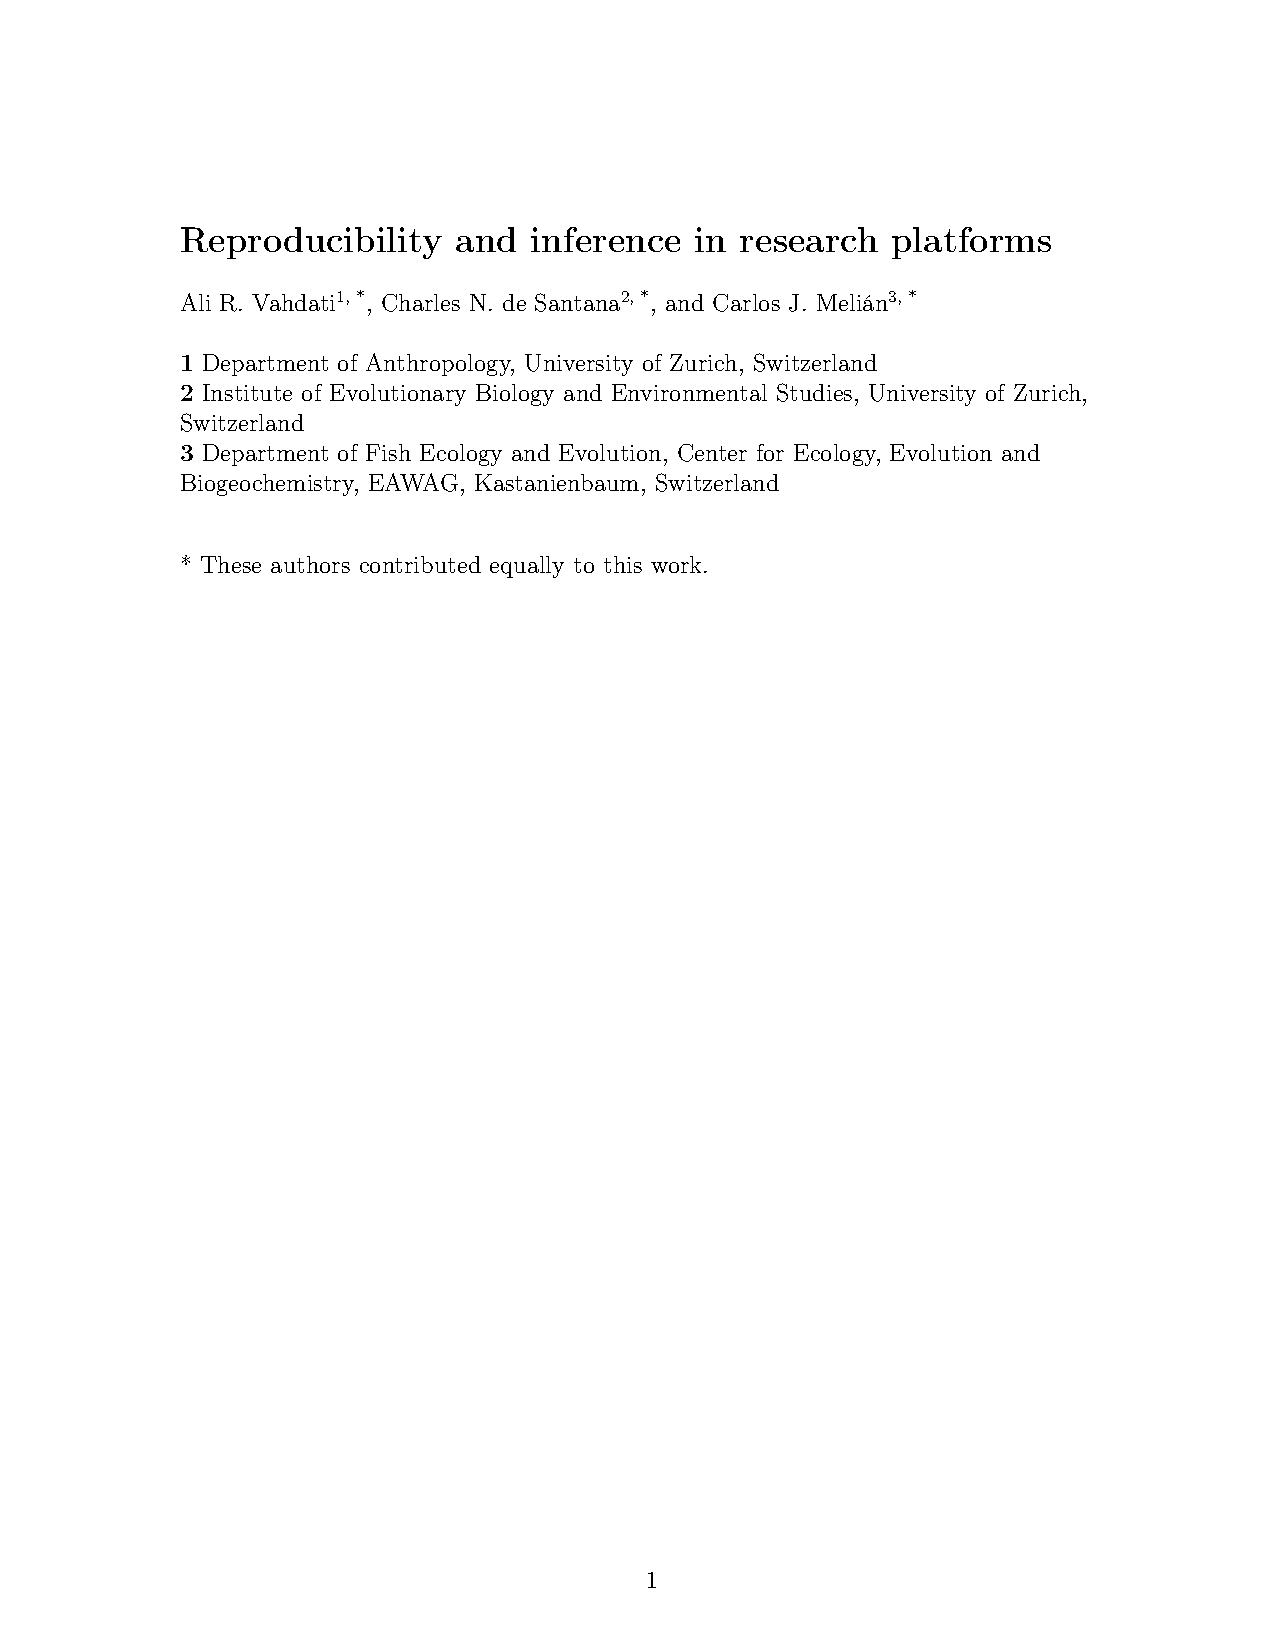
\includegraphics[scale=0.4]{robhoot.pdf}
\end{center}
\caption{Our dream icon $\mathcal{ROBHOOT}$}
\end{figure}
\end{flushleft}

\newpage
\carlos{PUNTOS A SOLUCIONAR\\
  \\
  \\
  1) Comparar codigos Modern Portfolio Theory para generar carteras. Usando como ejemplo el archivo Stocks.mat seleccionar N carteras con 20 stocks cada una. Coinciden las carteras? (Viernes 29 de Enero)
  \\
  2) Primeras carteras sobre Abril Mayo 2016. Incluidas diversificacion geografica y transicion entre carteras para minimizar comisiones
  \\  
  3) Cuenta de saxobank ya creada y el primer deposito de 12000USD hecho
  \\
  4) Lo ideal seria tener un manual avanzado del package ROBHOOT a finales del 2016. A partir de entonces se podria poner en github. Mientras seria ideal ir subiendo todo al server de sharelatex.
  \\
  5) Comparar codigos de julia y octave usando los dos quandl. Porducen el mismo output? Lo ideal seria compararlos todos. 
  \\
  6) Listado de productos de saxobank. Mirar en Quandl si solo con los nombres del pais ya sepuede acceder al listado de todos los productos. Consultar con Adrian de saxobank si existe ya el listado.
  }}

\newpage


\tableofcontents
\newpage

\section{Summary}

Investment markets are highly regulated and free access to
high-resolution data and investment models to accurately track market trends remains a challenge. Most companies offering services to small investors show a trade-off between free individual investment decisions at high fee
rates and decreasing investment cost at the expense of freedom (i.e.,
automated investments). Here we present the package $\mathcal{ROBHOOT}$ in julia to join free access to high-resolution data with a suite of investment models in one open access platform to investigate markets. Our goal is to allow small investors to access and combine fast and free worldwide high-resolution data and models to inform free-individual decisions and automated algorithms to track highly diversified portfolios.
\\
\\
Keywords: automated investments, approximate Bayesian computation,
regulatory markets, time series, informed individuals, complete
information, stochastic portfolio theory,
\newpage

\begin{comment}
\section{Investigating and investing in highly regulatory markets}

Strong resource dependence is a trade-off. One one side, obtaining all
resources from one labour and employer may help to make us more
specialized and efficient in completing some tasks. On the other side,
it may monopolize the surplus produced by individual's well oriented
ideas, risk and merit. Here we aim to facilitate informed portfolio
diversification for individuals that want to diversify risk and
merit. Any risk and merit fall within regulatory markets. Regulatory
markets control individual decisions to investigate for low cost a
worldwide connected and distributed market. Thus, it is important to
know the meaning of a regulatory market when diversifying
portfolios. In addition, we have to know how new ideas are being
developed in a highly regulatory market to overcome the high cost of
investments for small investors.
\end{comment}

\section{Open access to the data in a highly regulated market}


{\bf Introduce Quandl access to the data in julia: pros and cons}

Most networks, from genomes to ecosystems and markets of any kind are
highly regulated. This means most interacting agents in the market
have to deal with a highly complex set of regulations before having
access to the data, algorithms and the available strategies. Having
``easy'' access to the information in a ``perfectly informed market''
should be simple and efficient, but unfortunately, it is not. 

The first thing to consider is to have access to the data in a regulatory market. 
In order to get the data, we should know each product ID (e.g., as ID's for
species), the many to one tickers underlying each ID and how these
ID's apply to the products ranging from bonds to stocks\footnote{Link
  showing a full description of the available investment
  products}. There have been attempts to produce an ID following
international standards
\footnote{International Securities Identification Number, ISIN, \url{http://www.isin.org/isin-process/}}
\index{International securities identification number (ISIN)} (Figure
1 and 2). Each ID contains a time series, how and why each ID
fluctuate in a given market? How are markets connected? Which are the
underlying mechanisms producing the fluctuations and the correlations
between products and markets? Are highly correlated markets only
occurring in severe crisis? How regulatory markets influence
individual decisions to have free access to investigate and invest for
low or no cost in a worldwide connected and distributed market? Does
regulation mean higher cost to access the data and invest? Which is
the best (e.g., lowest cost?) strategy to invest in highly regulatory
markets?

The first step to answer these questions is to have easy and universal access to the data is a first step and there are a few attempts for such universal ID's. For example, the $Bloomberg$ $Open$ $Symbology$ data since 2012 contains a global and universal ID for each product and it allows to mappings to exchange tickers, ISINs and other financial data resources \footnote{Bloomberg open symbology, \url{http://datahub.io/dataset/bsym} and \url{https://github.com/ga-group/bsym}}. With the open symbology, obtaining high-resolution and free intra- and inter-day data in an integrated platform with access to all the markets should be easier but still the services offering data access and tracking the
market vary greatly and there are no options to have free and open access to the data with a global ID (\footnote{attempts include jstock \url{http://jstock.org/}}. Products range from the more classical close investment platform \index{close
  investment platform} to \index{automated investment platforms} at low fee\footnote{\url{https://www.sigfig.com/site/#/home/am}}. Close investment platform describes funds and investment products offered by a bank or firm a client decides to choose, limiting individual choices to free tracking and investing and diversifying portfolios. 

It is important to distinguish an open investment platform
\index{open investment platform}, on the other hand, where investors
can choose to invest in other funds and vehicles offered by competitor
institutions and companies from open platform in computing \index{open platform in computing}
which refers to a fully documented external application programming
interfaces (API) that allow using the software to function in other
ways than the original programmer intended, without requiring
modification of the source code. Ideally, an open platform in
computing should directly be translated to an open access server where
you can register for free and modify or not the embedded codes to
track your own portfolio, have access to high-resolution data \index{high-resolution data}
and automated investment algorithms \index{automated investments algorithms}.

Most investors are of small size and invest with a low frequency and
high-fee environment \footnote{Have access to the invested-size
  distribution per individual investors}. Thus, returns are small and
can be quickly erased by fees and highly fluctuating markets. For
example, investing in stocks can be very costly if we trade
constantly, especially with a minimum amount of money available to
invest. Every time that we trade stock, either buying or selling, we
will incur a trading fee. Trading fees range from the low end of $10$
per trade, but can be as high as $30$ for some brokers. Remember, a
trade is an order to purchase shares in one company. If we want to
purchase five different stocks at the same time, this is seen as five
separate trades and we will be charged for each one. Now, let's
imagine that we decide to buy the stocks of five companies with an
initial 10,000USD. To do this we will incur from 50USD to 150USD in
trading costs, which is equivalent to 0.5\% to 1.5\% of the initial
10,000USD. If we were to fully invest the 10,000, our account would be
reduced to 9950USD or 9850USD after trading costs. This represents an
important loss, before our investments even have a chance to earn a
cent. In addition, if we were to sell these five stocks, we would once
again incur the costs of the trades, which would be another 50USD or
150USD. To make the round trip (buying and selling) on these five
stocks it would cost us 100USD or 300USD, or 1\% or 3\% of our initial
deposit amount of 10,000USD. If our investments do not earn enough to
cover this, we have lost money by just entering and exiting positions
(the 10,000USD is far beyond what most small investors have to start
with!). In addition, hidden costs are the norm and most regulations
underlying investing should be explored further. 

\subsection{Keeping a balance between our ideas and worldwide distributed ideas}

There are millions of ideas fluctuating out there. Do most of them go
to extinction quickly? Diversifying portfolio in science and everyday
life is a simple consequence of living in fluctuating (and
unpredictable) environments. The closer we are at predicting
fluctuations of several time series (including your ideas) at local
and regional scales the better we know the ecosystem. Unfortunately,
it is not easy to predict time series of a large number of interacting
(ideally independent) species (or ideas or market products from stocks
to bonds). Given we can not predict most of the ideas' trends, we
should build a minimum understanding on how to investigate ideas and
build a diversified portfolio with a balance between risk and
reward. Basic questions will always remain when discussing about
predicting the future and diversifying portfolios. For example, in a
complex ecosystem, which is the best strategy under complete
ignorance? And under complete information? Should we invest following
a random walk \index{random walk}? Should we produce a portfolio with neutral risk
\index{neutral risk}?
\footnote{\url{https://en.wikipedia.org/wiki/A$_$Random$_$Walk$_$Down$_$Wall$_$Street}}

\section{Current portfolio theory in economics and ecology}

Portfolio theory in economics has a long tradition
\citep{MarkowitzBook}. The theory is rooted in the concept of efficient frontier\index{efficient frontier}. There are several companies and packages offering codes in several languages to calculate efficient frontiers\footnote{\url{http://www.quantcode.com/}}$^{,}$\footnote{\url{https://github.com/JuliaQuant/PortfolioModels.jl}}$^{,}$\footnote{\url{https://www.wikinvest.com/account/portfolio/register}}$^{,}$\footnote{\url{https://d1so5k0levrfcn.cloudfront.net/SigFig\%20Investment\%20Methodology.pdf}} . Most maths underlying portfoliio theory\index{portfolio theory} are based in matrix correlation patterns\index{matrix correlation patterns}. In ecology, portfolio concept has also been used to predict the number of coexisting species in landscapes with highly fluctuating environments\footnote{Check references}.

\subsection{Developing a highly diversified portfolio in time and space}

Given the basic maths underlying the portfolio theory, which are the
algorithms and models out there? Which one perform the best? Which is
the mixed of models to develop our investment strategy? Should we just
maximize reward and minimize risk (or volatility\index{volatility}) regardless
the frequency of trading? How to achieve it? How do frequency of
trading relate to maximum reward and minimum risk strategy? How to
connect a highly diversified portfolio with the knowledge of the
worldwide flow distribution of basic goods?\footnote{Check Bern
  principles}

\newpage
\section{Exploring de-centralized investments}

\subsection{Centralized investments}

The meaning of a centralized investment. Which are the pros and cons? Why centralized?

\subsection{Decentralized investments and virtual currency}

The meaning of decentralized investment. The origin of bitcoin and
refs to invest in virtual currencies.

\newpage
\section{Open platform to investigate markets ($\mathcal{ROBHOOT}$)}

In the long term, $\mathcal{ROBHOOT}$ will be a semi-automated investment tool combining
access to high-resolution data for both centralized and decentralized
investments, and free-individual decisions in individual products. To achieve such a combination, we aim to
develop $\mathcal{ROBHOOT}$ in two stages. The first stage will be to
develop the free-access platform to have access to the high-resolution
data to investigate markets (Figures 1 and 2). The second stage will
be to develop the steps required to allow individuals to invest
(Figure 3). There are several bottlenecks to develop such
platform. Enumerating these bottlenecks to recognize our lack of
expertise is a key first step. At this stage, there are at least 8
bottlenecks.

\subsection{Models}

\begin{comment}
1) Él ha analisado series temporales de stocks del mercado brasileiro con muestras a
 diferentes escalas temporales (semanales, diárias, intraday de 10 minutos)
2) Él ha comparado modelos linales, no lineales basados en maquinas de vectores de suporte, y modelos híbridos.
3) Ha dicho que modelos híbridos generan mejores predicciones de volatilidad que los demás modelos
4) No hay diferencia significativa entre los modelos no lineales que él estudió y los modelos lineales
5) La combinación de modelos que genera menos errores es utilizar modelos *lineales* para 
predecir los valores esperados y los modelos *hibridos* para predecir la volatilidad
6) Ha dicho que la principal limitación de los modelos que ha estudiado es que los errores
 (los componentes aleatorios) son muy altos cuando comparaods a los componentes determinísticos. 
 Además de eso, la varianza de los componentes aleatorios cambia a lo largo del tiempo, lo que hace mucho dificil la predicción.
7) Ha dicho que los modelos de black-Litterman utilizan la matriz de covarianza y posiblemente
 tendrán la misma limitación en la predicción que los modelos que él ha estudiado en su master 
 (él no conocía el Black-Litterman, pero ha mirado el paper que Carlos nos envió y me lo dijo).
8) El artículo que envié anteriormente, que habla de la predicción de Bitcoin, también 
utiliza la matriz de covarianza. Pero Gilmar cree que dicha predicción solo fué posible 
porque ellos utilizan informaciones del "libro de ofertas", que resulta 
en un valor entre -1 y 1. Si el valor es -1, significa que todos en el mercado solo quieren vender.
 Si el valor es +1, siginifca que todos solo quieren comprar. Ha dicho que es tipo de información
  es dificil para el mercado de stocks. Creo que allí entramos nosotros! ;)
10) Por esa razón, él cree que es dificil hacer predicciones fiables del comportamiento de stocks. 
Por eso cree que lo mejor es estudiar el riesgo de los stocks, en vez de la predicción.
11) Ha dicho que para su doctorado, él va a utilizar solamente modelos lineales, porque ha dicho 
que lo que se gana con los modelos no hibridos no le parece suficiente como para perder en 
la performance de la simulación. Su objetivo es intentar mejorar la limitación que mencioné anteriormente.
\end{comment}

\subsection{Pattern detection models}

\subsubsection{Modern Portfolio Theory}

Explain briefly the main assumptions and the main albegra used. 
Mention the matlab and julia codes with access to quandl data.

\subsubsection{Mixed Estimation Model: Black-Litterman model}

The Mixed Estimation Model was developed by Henri Theil in the early 1960's, but was applied to financial data by Fischer Black and Robert Litterman in the early 1990's. The beauty of this model is that one can blend a variety of views specified in different ways, absolute or relative, with a given prior estimate to generate a new and updated posterior estimate which includes all the views. The updated posterior estimate should be centered more closely around the unknown mean, and should also have a lower variance(higher precision) that either the prior or conditional distribution. There are implementations in matlab\footnote{\url{http://www.blacklitterman.org/intro.html}} and new automated investment companies use the Black-Litterman model for their automated decisions\footnote{\url{https://www.betterment.com/resources/investment-strategy/why-you-should-invest-beyond-us-stocks/}}. $\mathcal{ROBHOOT}$ uses the matlab version from\footnote{\url{http://www.blacklitterman.org/intro.html}} implemented in julia. 


\subsubsection{Neural network model}

\subsubsection{Elliott waves model}


\subsection{Dynamic or mechanistic models}

\subsubsection{Brownian motion model (Random walk model)}



\section{Bottlenecks}

\subsubsection{Bottleneck 1: Data access algorithms}

Streaming data analysis will be the key when accessing the data. Investment products datasets are too large to store in RAM and are being generated in real time. 


Bottleneck 1 would require to retrieve ID's from the Bloomberg open symbology\footnote{Methods to convert each product between their ID's. For example, convert 9-digit CUSIP codes into ISIN codes \url{http://stackoverflow.com/questions/30545239/convert-9-digit-cusip-codes-into-isin-codes}}. This is not just connecting algorithms to google or yahoo to have access to interday data for a few markets and products (this is by far a trivial problem). Data access has, at least, three steps: 1) ID database access using open symbology; 2) link ID to the several stickers each ISIN contains with a different sticker name in each different market (ID or ISIN can be
compared with the genome of each investment product and the stickers would be the different varieties of a species in space), and 3) connect the ID or ISIN to the time series at high (intraday) or low
(interday) resolution with price and volume values. TODAY, THERE IS NO SERVER OFFERING THIS EASY ACCESS SERVICE FOR FREE FOR ANY PRODUCT IN ANY MARKET.

\subsubsection{Bottleneck 2: Pattern detection algorithms}

Bottleneck 2, pattern detection, includes several open problems but
they can mostly be reduced to one. This is to have a solid background
in stochastic portfolio theory \index{stochastic portfolio theory} to build a codebase \index{codebase}
from the most simple one investment product to several investments
products. The codebase should be ready to simulate the efficient
frontier for any given portfolio.

\subsubsection{Bottleneck 3: Mechanistic model algorithms}

Bottlenecks in step 3 are those based in model development, selection
and inference. Complex models will be difficult to analyze using
Approximate Bayesian computation methods to develop diversified
investment strategies. Thus, combining our own (complex) decisions
with the available algorithm and methods should allow to simplify the
models and run ABC to compare them before developing the strategies to
invest.

\subsubsection{Bottleneck 4: Validation and ABC algorithms}

\subsubsection{Bottleneck 5: Automated decision algorithms}

\subsubsection{Bottleneck 6: API development, cloud access and counting metrics}

\subsubsection{Bottleneck 7: Open platform in a highly regulatory market}

\subsubsection{Bottleneck 8: Security and encryption methods}



\newpage
\section{Acknowledgments}


\newpage
\bibliographystyle{evolution}
\bibliography{ref}

\newpage

\section{Tables}


\newpage

\section{Figures}

%Figure 1: TRADE-OFFS: Individual decisions at high cost and automated decision at low cost (Why not both?)


%Figure 2: ROBHOT: Steps to develop ROBHOT
\begin{figure}
\vspace{-1 in}
\begin{center}
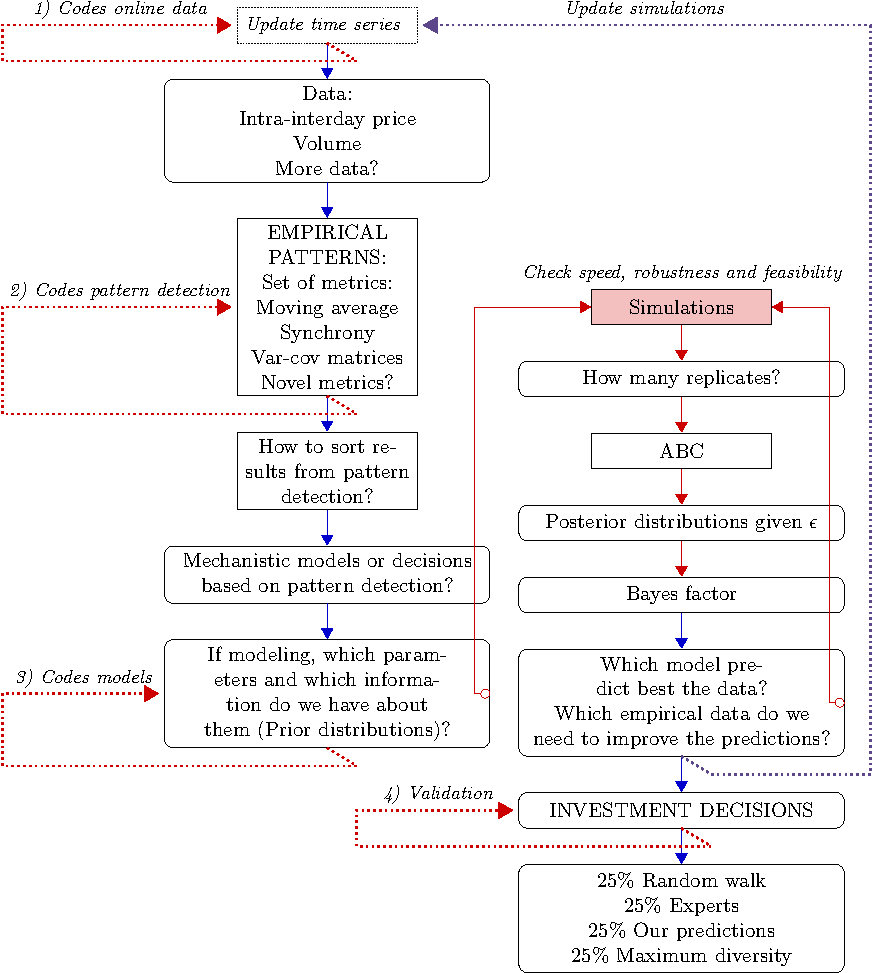
\includegraphics[scale=0.8]{EasyFlowChart.pdf}
\end{center}
\caption{Flow chart summarizing the steps to develop $\mathcal{ROBHOOT}$}
%\label{}
\end{figure}
\newpage

%Figure 3: ROBHOT: Steps to develop ROBHOT
\begin{figure}
\vspace{-1 in}
\begin{center}
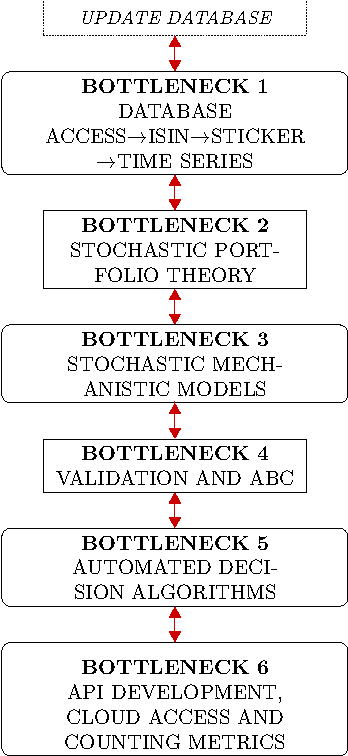
\includegraphics[scale=1.25]{EasyFlowChartBottlenecks.pdf}
\end{center}
\caption{Bottlenecks to overcome to develop $\mathcal{ROBHOOT}$}
\end{figure}
\newpage

%Figure 3: ROBHOT: Steps to develop ROBHOT
%\begin{figure}
%\vspace{-1 in}
%\begin{center}
%\includegraphics[scale=0.8]{EasyFlowChartOPTIIMA.pdf}
%\end{center}
%\caption{Flow chart summarizing the steps to develop ROBHOT (phase II)}
%\label{}
%\end{figure}

\printindex
\end{document}
